\subsection{Karakteristike sistema}
Prilikom razmatranja arhitekture informacionog sistema cilj je bio napraviti jednostavnu, shiroko dostupnu, stabilnu i bezbednu aplikaciju. Izborom veb aplikacije obezbedili smo shiroku dostupnost jer je za njeno korish\c1enje potrebno samo da korisnik ima
internet vezu na svom rachunaru. Pazhljivo vodec1i rachuna prilikom izrade korisnichkog
interfejsa je postignuta jednostavnost a stabilnost i pre svega bezbednost izborom
troslojne arhitekture gde se sredishnji (logichki) sloj deli na klijentski i serverski deo.
Karakteristike arhitekture sistema za transport shec1era:
\begin{enumerate}
    \item  Tip aplikacije: Veb aplikacija
    \item Strategije isporuchivanja: Jedan serverski i vishe klijent\-skih rachunara
    \item Tehnologije: $PHP$, $HTML$, $Javascript$
    \item Pratec1e komponente:

    \begin{enumerate}
        \item  Logovanje na sistem: Podsistem za autentikaciju korisnika
        \item Pomoc1: Uput\-stvo za korish\-c1enje veb aplikacije, kontakt forma, $FAQ$
        \item Pravljenje kopije baze podataka: Podsistem koji automatski ili na zahtev pravi kopiju baze podataka
        \end{enumerate}

\end{enumerate}
Na slici \ref{fig:arh} se nalazi predlog arhitekture sistema.

\begin{figure}[H]
    \centering
    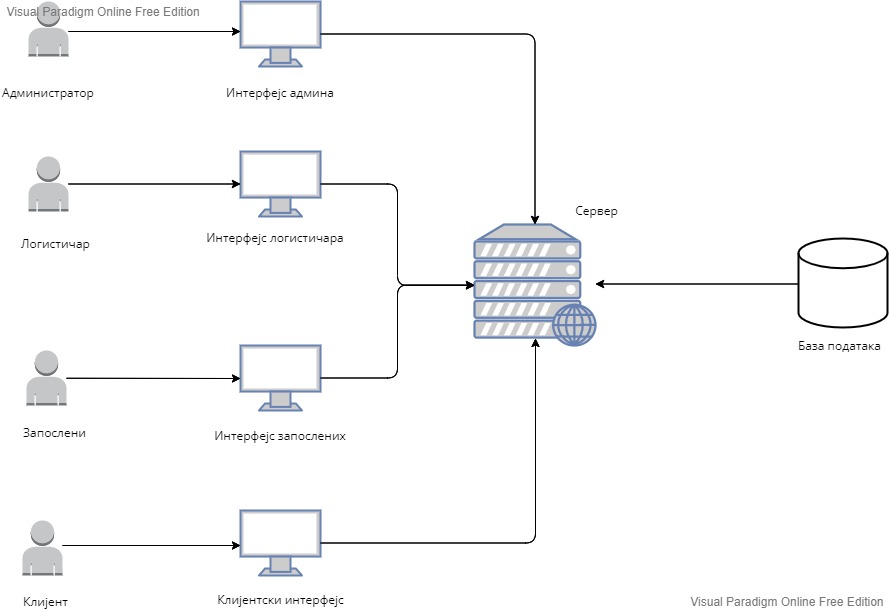
\includegraphics[width=12cm]{Slike/Arhitektura/arhitektura .jpg}
    \caption{Predlog arhitekture}
    \label{fig:arh}
\end{figure}



\subsection{Tip i slojevi arhitekture}
Arhitektura informacionog sistema je zamishljena kao klijent - server arhitektura i
sastoji se iz tri sloja pri chemu se sredishnji sloj deli na dve komponente: 
\begin{itemize}
    \item  Prezentacioni sloj
\item Logichki sloj
\begin{itemize}
    \item Klijent kontroler
    \item Server kontroler
\end{itemize}

\item Sloj podataka

\end{itemize}
Na slici \ref{fig:klijent-server} se nalazi dijagram klijent-server arhitekture.


\begin{figure}[H]
    \centering
    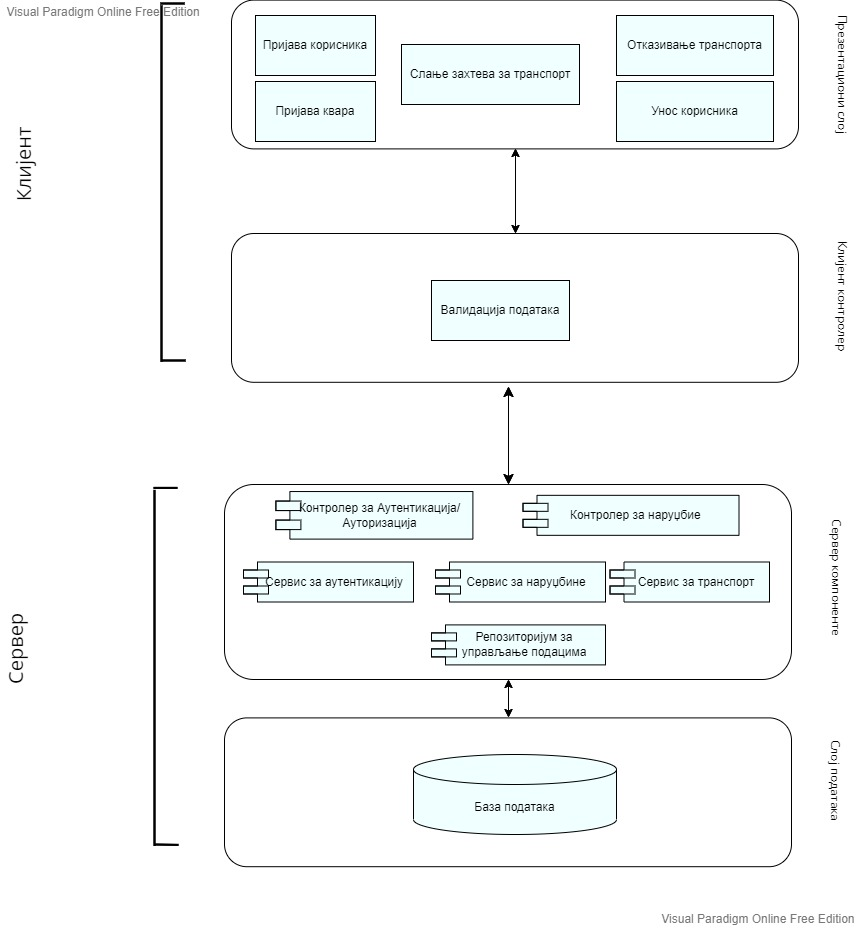
\includegraphics[width=12cm]{Slike/Arhitektura/predlogArhitekture.jpg}
    \caption{Klijent server arhitektura sistema}
    \label{fig:klijent-server}
\end{figure}

\subsubsection{Komponente klijenta}
\begin{enumerate}
    \item \textbf{Prezentacioni sloj}
    Predstavlja najvishi sloj aplikacije i ima ulogu da korisniku
prikazhe vizuelnu reprezentaciju sadrzhaja na osnovu podataka koje dobija od nizheg
sloja. Sastoji se od skupa $html$ stranica koje su izgrađene uz pomoc1 $HTML$, $CSS$, a njihov detaljan izgled c1e biti prikazan u narednom poglavlju. Pochetna stranica je $index.html$ na kojoj korisnik vrshi prijavu na sistem i ima moguc1nost naruchivanja ili otkazivanja transporta. 
\end{enumerate}
\subsubsection{Komponente servera}
\begin{enumerate}
    \item {\textbf{Kontrolerski sloj}}
			Predstavlja logicki sloj servera i ima ulogu u primanju zahteva koje klijent sloj shalje kao i odgovaranje na iste. U okviru ovog sloja nalazi se i biznis logika celog sistema.  Implementacija ovog sloja je izvrshena pravljenjem otvorenog $API$-ja (\fontencoding{T1} \selectfont Application programming interface \fontencoding{OT2} \selectfont ) ka korisnichkom sloju sa upotrebom $RESTFul$ konvencije. Realizacija implementacije saderzhac1e $PHP$ skripte koje c1e u odnosu na zahtev dobijen od strane klijentske strane obrad1ivati dobijene podatke i stupati u kontakt sa slojem podataka kada to bude potrebno. Za implementaciju koristicemo \fontencoding{T1} \selectfont Controller-Service-Repository\fontencoding{OT2} \selectfont  model.  Komponente koje c1e biti raspolozhive sistemu su:
			\begin{itemize}
				\item {\textbf{Kontroler za Autentikaciju(Autorizaciju)} \\
						Ovaj kontroler prima sve vrste zahteva po pitanju logovanja. Klijenska strana c1e kroz razlichite forme omoguc1iti korisniku ovog sistema da svoje podatke za logovanje prosledi ovom kontroleru (korish\-c1enjem $API$-ja) . Nakon chega se iz skupa moguc1ih lokacija korisnik prosled1uje u zavisnosti od njegovih privilegija pristupa.}
				\item{\textbf{Servis za autentikaciju}\\
				Biznis logika iza celog procesa autentikacije. Nakon odred1enih autentikacija vrac1a informaciju kontroleru o tome koja su prava pristupa klijenta, i da li ih uopshte i ima, naravno.}
				\item{\textbf{Kontroler za narud2bine}\\
					To je kontroler koji je zaduzhen za primanje zahteva vezanih za narud2bine kao i za validaciju istih.  Ovaj kontroler c1e biti povezan sa servisom za rute, kao i sa servisom sa narudzbine. }
				\item{\textbf{Servis za narud2bine} \\
					U njemu se nalazi sva biznis logika obrade, validacije i potvrde narudzbina i u komunikaciji je sa repozitorijumom za upravljanje podataka}
				\item{\textbf{Servis za transport} \\
					Servis u kome se nalazi sva bizinis logika vezana za transport i rutem, npr logika biranja ruta}
				\item{\textbf{Repozitorijum za upravljanje podacima}
					S obzirom na malu kolichinu podataka kojima raspolazhemo, dovoljno je da imamo samo jedan repozitorijum koji je na najnizhem sloju nashe aplikacije povezan sa bazom podataka iz koje izvlachi potrebne podatke kao i azhurira postojec1e }
			\end{itemize} 
		Kontroleri koji se nalaze u nashem sistemu bic1e zhargonski recheno gad1ani od strane klijentske strane po rutama koje c1e ti kontroleri definisati, usled razlichitih privilegija koje korisnici sistema mogu imati, nece sve rute kontrolera biti dostupne svima.  Kontroleri ni u jednom trenutnku nec1e biti direktno u komunikaciji sa repozitorijumom, a naravno ni sa bazom podataka. Kontroleri nasheg sistema c1e nakon prosled1ivanja podatka i zadataka servisima, nakon izvrshenih radnji i odgova istih, nazad klijentkoj strani slati informaciju o tome da li je akcija bila uspeshna i shta je rezultat trazhene akcije.
	
	\item{\textbf{Sloj podataka}} \\
		Tabele koje c1e se nalaziti u ovoj bazi podataka opisane su dijagramom klasa. Podaci c1e biti skladishteni u memoriji na serverskom rachunaru, i to u $Postgres$ bazi podataka. Jedini nachin pristupa bazi podataka bic1e preko repozitorijuma koji je ujedno i najnizhi nashe aplikacije, dok c1e repozitorijum biti povezan sa bazom podataka preko odred1enih komponenti okruzhenja ($Framework$), jedno takvo okruzhenje za $PHP$ bi bio $Laravel$ koji nudi jednostavno povezivanje . 
		
\end{enumerate}

